%!TEX root = ../diss.tex
\tikzstyle{element}=[rectangle, thick,
                     inner sep=0.1cm, rounded corners]
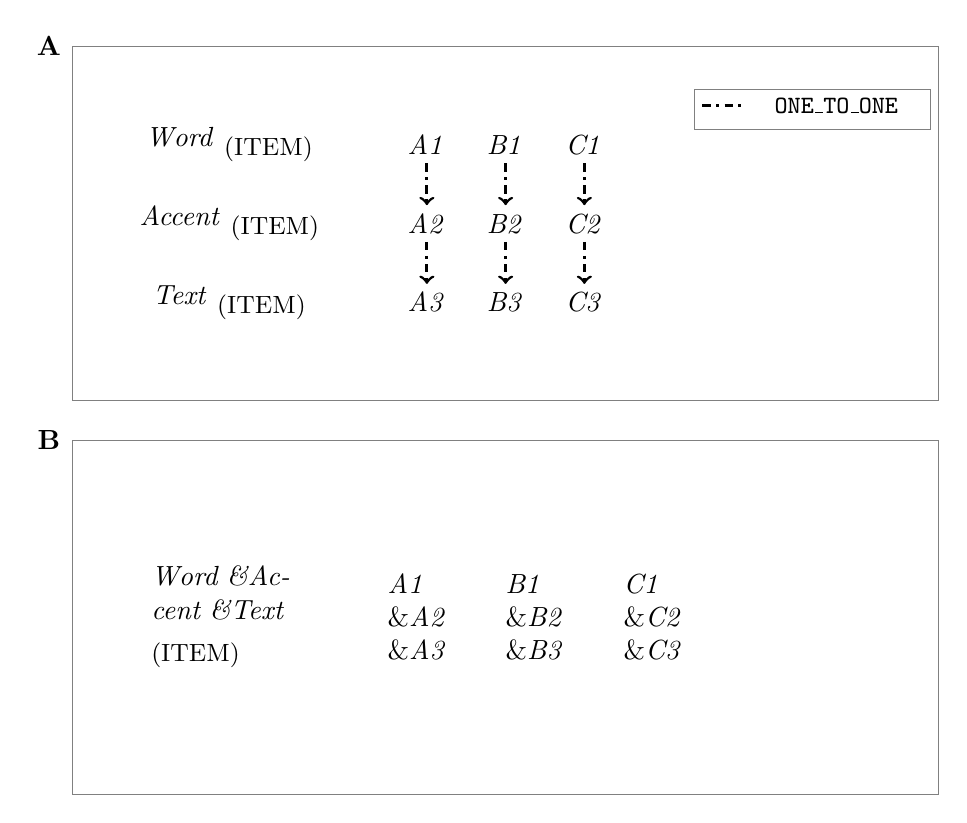
\begin{tikzpicture}

%%%%%%%%%%%%%%%%%%%%%%%%%%%%%%
% nodes

% A
\draw[gray] (-5.5, 9.75) rectangle (5.5, 5.25);
\node (a) at (-5.8, 9.75){\textbf{A}};

\node (w_A) at (-3.5, 8.5) [element] {\textit{Word} \textsubscript{\small{(ITEM)}}};
\node (a_A) at (-3.5, 7.5) [element] {\textit{Accent} \textsubscript{\small{(ITEM)}}};
\node (t_A) at (-3.5, 6.5) [element] {\textit{Text} \textsubscript{\small{(ITEM)}}};

\node (A1_A) at (-1, 8.5) [element] {\textit{A1}};
\node (A2_A) at (-1, 7.5) [element] {\textit{A2}};
\node (A3_A) at (-1, 6.5) [element] {\textit{A3}};

\node (B1_A) at (0, 8.5) [element] {\textit{B1}};
\node (B2_A) at (0, 7.5) [element] {\textit{B2}};
\node (B3_A) at (0, 6.5) [element] {\textit{B3}};

\node (C1_A) at (1, 8.5) [element] {\textit{C1}};
\node (C2_A) at (1, 7.5) [element] {\textit{C2}};
\node (C3_A) at (1, 6.5) [element] {\textit{C3}};


% complex
\draw[gray] (-5.5, 4.75) rectangle (5.5, 0.25);
\node (b) at (-5.8, 4.75){\textbf{B}};

\node (wat_B) at (-3.5, 2.5) [element, text width = 2cm] {\textit{Word \&Accent \&Text} \textsubscript{\small{(ITEM)}}};

\node (A123_B) at (-1, 2.5) [element, text width = 1cm] {\textit{A1} \&\textit{A2} \&\textit{A3}};

\node (B123_B) at (0.5, 2.5) [element, text width = 1cm] {\textit{B1} \&\textit{B2} \&\textit{B3}};

\node (C123_B) at (2, 2.5) [element, text width = 1cm] {\textit{C1} \&\textit{C2} \&\textit{C3}};

%%%%%%%%%%%%%%%%%%%%%%%%%%%%%%
% legends

% A
\draw[gray] (2.4, 9.2) rectangle (5.4, 8.7);
\node (leg_simp_o2m) at (4.2, 9) [element] {\small{\texttt{ONE\_TO\_ONE}}};
% \node (leg_sim_m2m) at (4.2, 8.5) [element] {item seq.};
\draw [-, line width=1, dashdotted] (2.5, 9) to (3.0, 9);
% \draw [->, line width=1] (2.5, 8.5) to (3.0, 8.5);


% B
% \draw[gray] (2.4, 4.2) rectangle (5.4, 3.6);
% \node (leg_simp_o2m) at (4.2, 3.9) [element] {item seq.};
% \draw [->, line width=1] (2.5, 3.9) to (3.0, 3.9);

%%%%%%%%%%%%%%%%%%%%%%%%%%%%%%
% links

% A
\draw [->, line width=1, dashdotted] (A1_A) to (A2_A);
\draw [->, line width=1, dashdotted] (A2_A) to (A3_A);

\draw [->, line width=1, dashdotted] (B1_A) to (B2_A);
\draw [->, line width=1, dashdotted] (B2_A) to (B3_A);

\draw [->, line width=1, dashdotted] (C1_A) to (C2_A);
\draw [->, line width=1, dashdotted] (C2_A) to (C3_A);

% \draw [->, line width=1] (A1_A) to (B1_A);
% \draw [->, line width=1] (B1_A) to (C1_A);
% 
% \draw [->, line width=1] (A2_A) to (B2_A);
% \draw [->, line width=1] (B2_A) to (C2_A);
% 
% \draw [->, line width=1] (A3_A) to (B3_A);
% \draw [->, line width=1] (B3_A) to (C3_A);

% B
% \draw [->, line width=1] (A123_B) to (B123_B);
% \draw [->, line width=1] (B123_B) to (C123_B);

\end{tikzpicture}
